%!Tex Root = ../Vorlage_Uebungsblatt.tex
% ./Packete.tex
% ./Design.tex
% ./Deklarationen.tex
% Kapitel2

\if\thesis1\chapter{Kapitel 1}\label{ch:kapitel1}\fi

\begin{table}[H]
  \center
  \begin{NiceTabular}{X[1,c]X[2,l]}[rules/color=PrimaryColor] % {\linewidth}{|C|C|L|L|}
    \CodeBefore
    \chessboardcolors{white}{BoxColor}
    \rowcolor{PrimaryColor}{1}
    \Body
    \textcolor{white}{\textbf{Spalte 1}} & \textcolor{white}{\textbf{Spalte 2}} \\
    \smalltt{row1} & \colorbold{Beschreibung} für \smalltt{row1}. \\
    \smalltt{row2} & \acolorbold{Beschreibung} für \smalltt{row2}. \\
    \bottomrule
  \end{NiceTabular}
  \caption{Beispiel.}
\end{table}

\begin{figure}
  \begin{transformation}[0.3][0.4]
    {\dq}{4}\enspace {*}\enspace {2}{\dq}
    \arrowxx{Aktion 1}{Aktion 2}
    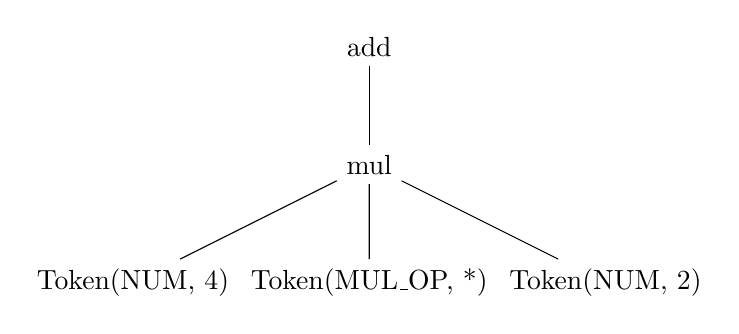
\begin{tikzpicture}[auto, align=center, sibling distance=3cm, level distance=1.5cm, baseline=(current  bounding  box.center)]
      \node {\smalltt{add}}
      child {node {\smalltt{mul}}
        child {node {\smalltt{Token(NUM, \dq 4\dq)}}}
        child {node {\smalltt{Token(MUL\_OP, \dq *\dq)}}}
        child {node {\smalltt{Token(NUM, \dq 2\dq)}}}};
    \end{tikzpicture}
  \end{transformation}
  \caption{Untertitel.}
\end{figure}

\begin{itemize}
  \item asdf
  \item asdf
  \begin{itemize}
    \item asdf
    \aitem asdf
    \greyitem asdf
  \end{itemize}
\end{itemize}

\begin{equation}
  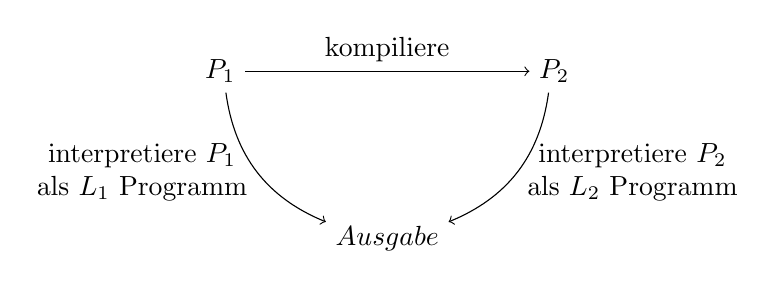
\begin{tikzpicture}[auto, baseline=(current  bounding  box.center)]
    \node (program1) at (135:3) {$P_{1}$};
    \node (program2) at (45:3) {$P_{2}$};
    \node (output)  at (270:0) {$Ausgabe$};

    % https://tex.stackexchange.com/questions/24372/how-to-add-newline-within-node-using-tikz
    \draw[->] (program1) to node[above] {kompiliere} (program2);
    \draw[->] (program1) to[bend right] node[left, align=center] {interpretiere $P_{1}$\\ als $L_{1}$ Programm} (output);
    \draw[->] (program2) to[bend left] node[right, align=center] {interpretiere $P_{2}$\\ als $L_{2}$ Programm} (output);
  \end{tikzpicture}
\end{equation}

\begin{linenums}
  \numberedcodebox[remember as=codebeispiel, minted language=c, minted options={}]{./code_examples/example.c}
\end{linenums}

\codebox[title=Codebeispiel 2, remember as=codebeispiel_other, hbox, minted language=c, minted options={}]{./code_examples/example.c}

{
  \codebox[title=Codebeispiel 1, remember as=codebeispiel1, width=0.4\linewidth, nobeforeafter, minted language=c, equal height group=A, minted options={highlightlines={1, 3-7}}]{./code_examples/example.c}
  \hfill
  \codebox[title=Codebeispiel 2,  remember as=codebeispiel2, width=0.4\linewidth, nobeforeafter, minted language=c, equal height group=A, minted options={highlightlines={1, 3-7}}]{./code_examples/example.c}

  \begin{tikzpicture}[overlay,remember picture,line width=1mm, font=\small, draw=PrimaryColor]
    \draw[->] (codebeispiel1.east) to[bend left] node[above, align=center] {Mehrzeiliger\\ Text} (codebeispiel2.west);
  \end{tikzpicture}
}

% \begin{itemize}
%   \item \inlinebox{arg} aus \inlinebox*{command arg}.
%   \aitem \key{\Uparrow-Tab}.
%   \item longline longline longline longline longline longline longline longline longline longline longline longline.
%   \begin{itemize}
%     \item longline longline longline longline longline longline longline longline longline longline longline longline.
%     \grayitem \textcolor{gray!90!black}{test test test.}
%   \end{itemize}
% \end{itemize}
%
% % todo
% \begin{enumerate}
%   \item asdf
%   \item asdf
% \end{enumerate}
%
% {
%   \centering
%   \begin{file}[remember as=input]
%     Start
%   \end{file}
%   \vspace{0.1cm}
%   \begin{codeframe}*[remember as=frameone]{Frame 1}
%     \codebox[title=Codebeispiel 1, width=0.4\linewidth, nobeforeafter, minted language=text, equal height group=A, minted options={highlightlines={2}}]{./code_examples/example2.special}
%     \hfill
%     \codebox*[title=Codebeispiel 2, width=0.4\linewidth, nobeforeafter, minted language=text, equal height group=A, minted options={highlightlines={3}}]{./code_examples/example2.special}
%   \end{codeframe}
%   \vspace{0.1cm}
%   \begin{file}[remember as=conta]
%     ...
%   \end{file}
%   \begin{tikzpicture}[overlay,remember picture,line width=1mm,draw=PrimaryColor, font=\tiny]
%     \draw[->, color=SecondaryColor] (input.south) to node[right=0.25cm, align=center] {\textcolor{black}{Verbindung 1}} (frameone.north);
%     \draw[->] (frameone.south) to node[right=0.25cm, align=center] {Verbindung 2} (conta.north);
%   \end{tikzpicture}
% }
%
% \begin{terminal}
%   |\prompt| command arg
%   |\customprompt| command arg
% \end{terminal}
%
% \begin{Sidenote}
%   \begin{itemize}
%     \item test
%     \item test2
%   \end{itemize}
% \end{Sidenote}
